\documentclass{standalone}
\usepackage{tikz}
\usetikzlibrary{patterns, positioning}
\usepackage[sfdefault]{ClearSans} %% option 'sfdefault' activates Clear Sans as the default text font
\usepackage[T1]{fontenc}

\begin{document}
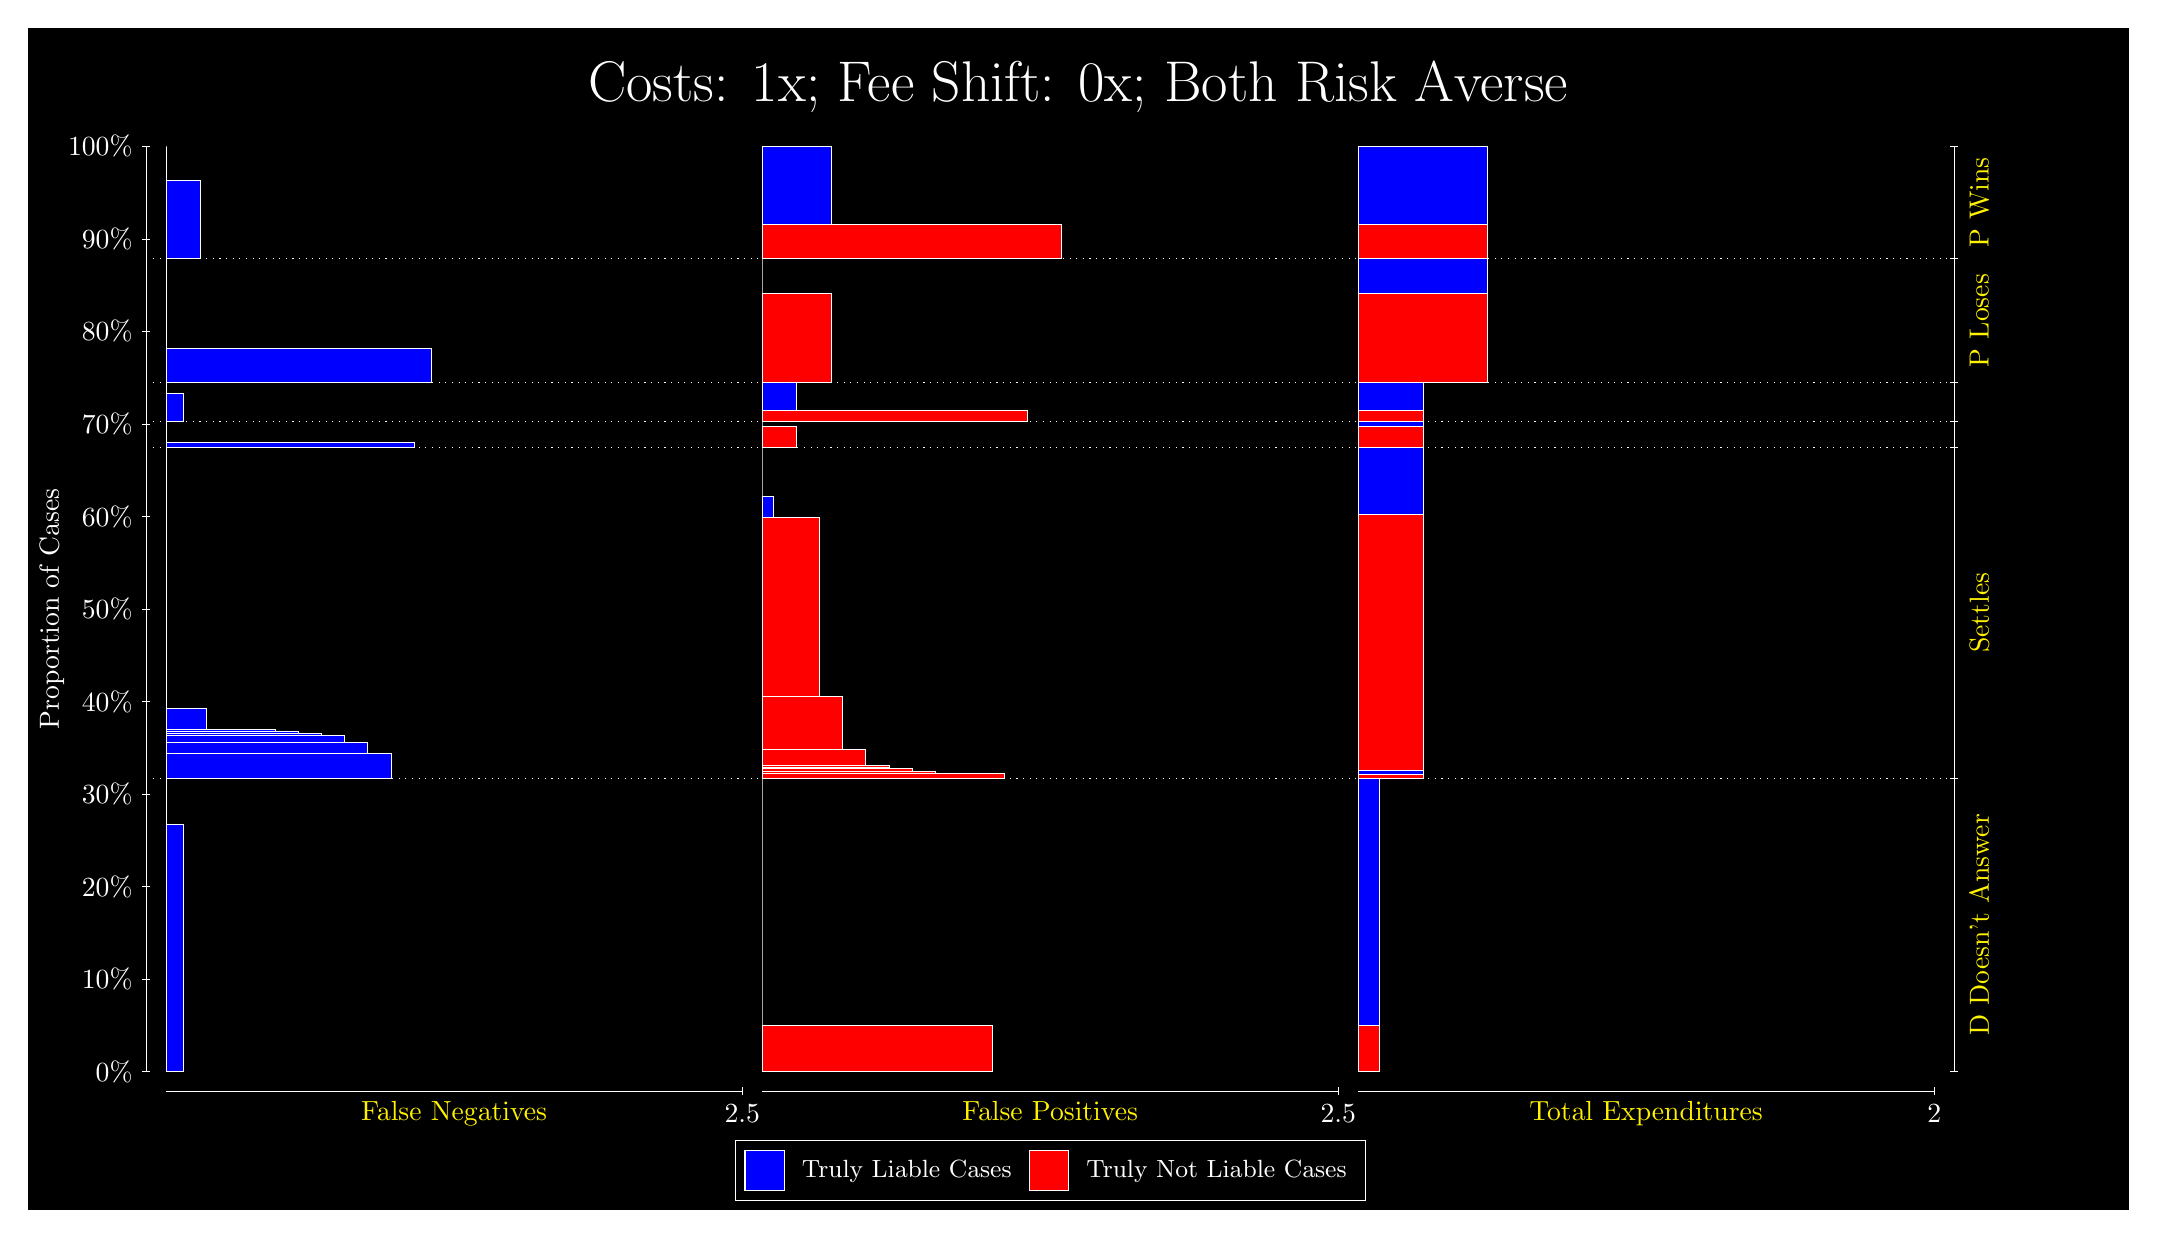
\begin{tikzpicture}
\draw[fill=black] (0,0) rectangle (26.667,15);
\draw[text=white] (0,13.5) rectangle (26.667,15) node[midway] {\huge Costs: 1x; Fee Shift: 0x; Both Risk Averse};
\draw[white, very thin] (1.5,1.75) -- (1.5,13.5);
\node[rotate=90, text=white, anchor=center] at (0.3, 7.625) {Proportion of Cases};
\draw[white, very thin] (1.45,1.75) -- (1.55,1.75);
\node[text=white, anchor=east] at (1.45, 1.75) {0\%};
\draw[white, very thin] (1.45,2.925) -- (1.55,2.925);
\node[text=white, anchor=east] at (1.45, 2.925) {10\%};
\draw[white, very thin] (1.45,4.1) -- (1.55,4.1);
\node[text=white, anchor=east] at (1.45, 4.1) {20\%};
\draw[white, very thin] (1.45,5.275) -- (1.55,5.275);
\node[text=white, anchor=east] at (1.45, 5.275) {30\%};
\draw[white, very thin] (1.45,6.45) -- (1.55,6.45);
\node[text=white, anchor=east] at (1.45, 6.45) {40\%};
\draw[white, very thin] (1.45,7.625) -- (1.55,7.625);
\node[text=white, anchor=east] at (1.45, 7.625) {50\%};
\draw[white, very thin] (1.45,8.8) -- (1.55,8.8);
\node[text=white, anchor=east] at (1.45, 8.8) {60\%};
\draw[white, very thin] (1.45,9.975) -- (1.55,9.975);
\node[text=white, anchor=east] at (1.45, 9.975) {70\%};
\draw[white, very thin] (1.45,11.15) -- (1.55,11.15);
\node[text=white, anchor=east] at (1.45, 11.15) {80\%};
\draw[white, very thin] (1.45,12.325) -- (1.55,12.325);
\node[text=white, anchor=east] at (1.45, 12.325) {90\%};
\draw[white, very thin] (1.45,13.5) -- (1.55,13.5);
\node[text=white, anchor=east] at (1.45, 13.5) {100\%};

\draw[white, very thin] (24.457,1.75) -- (24.457,13.5);
\draw[white, very thin] (24.407,1.75) -- (24.507,1.75);
\node[anchor=west] at (24.407, 1.75) {};
\draw[white, very thin] (24.407,5.4732) -- (24.507,5.4732);
\node[anchor=west] at (24.407, 5.4732) {};
\draw[white, very thin] (24.407,9.6789) -- (24.507,9.6789);
\node[anchor=west] at (24.407, 9.6789) {};
\draw[white, very thin] (24.407,10.008) -- (24.507,10.008);
\node[anchor=west] at (24.407, 10.008) {};
\draw[white, very thin] (24.407,10.5) -- (24.507,10.5);
\node[anchor=west] at (24.407, 10.5) {};
\draw[white, very thin] (24.407,12.072) -- (24.507,12.072);
\node[anchor=west] at (24.407, 12.072) {};
\draw[white, very thin] (24.407,13.5) -- (24.507,13.5);
\node[anchor=west] at (24.407, 13.5) {};

\draw[white, very thin, fill=blue] (1.75,1.75) rectangle (1.9696,4.8885);
\draw[white, very thin, fill=red] (1.75,4.8885) rectangle (1.75,5.4732);
\draw[white, very thin, fill=blue] (1.75,5.4732) rectangle (4.6044,5.798);
\draw[white, very thin, fill=blue] (1.75,5.798) rectangle (4.3116,5.9302);
\draw[white, very thin, fill=blue] (1.75,5.9302) rectangle (4.0188,6.0187);
\draw[white, very thin, fill=blue] (1.75,6.0187) rectangle (3.7261,6.0413);
\draw[white, very thin, fill=blue] (1.75,6.0413) rectangle (3.4333,6.0747);
\draw[white, very thin, fill=blue] (1.75,6.0747) rectangle (3.1406,6.0968);
\draw[white, very thin, fill=blue] (1.75,6.0968) rectangle (2.8478,6.0992);
\draw[white, very thin, fill=blue] (1.75,6.0992) rectangle (2.5551,6.1012);
\draw[white, very thin, fill=blue] (1.75,6.1012) rectangle (2.2623,6.3693);
\draw[white, very thin, fill=red] (1.75,6.3693) rectangle (1.75,9.6789);
\draw[white, very thin, fill=blue] (1.75,9.6789) rectangle (4.8971,9.7371);
\draw[white, very thin, fill=red] (1.75,9.7371) rectangle (1.75,10.008);
\draw[white, very thin, fill=blue] (1.75,10.008) rectangle (1.9696,10.362);
\draw[white, very thin, fill=red] (1.75,10.362) rectangle (1.75,10.5);
\draw[white, very thin, fill=blue] (1.75,10.5) rectangle (5.1167,10.935);
\draw[white, very thin, fill=red] (1.75,10.935) rectangle (1.75,12.072);
\draw[white, very thin, fill=blue] (1.75,12.072) rectangle (2.1891,13.065);
\draw[white, very thin, fill=red] (1.75,13.065) rectangle (1.75,13.5);
\draw[white, very thin, fill=red] (9.3189,1.75) rectangle (12.246,2.3347);
\draw[white, very thin, fill=blue] (9.3189,2.3347) rectangle (9.3189,5.4732);
\draw[white, very thin, fill=red] (9.3189,5.4732) rectangle (12.393,5.5368);
\draw[white, very thin, fill=red] (9.3189,5.5368) rectangle (12.1,5.5384);
\draw[white, very thin, fill=red] (9.3189,5.5384) rectangle (11.807,5.5407);
\draw[white, very thin, fill=red] (9.3189,5.5407) rectangle (11.515,5.5572);
\draw[white, very thin, fill=red] (9.3189,5.5572) rectangle (11.222,5.6033);
\draw[white, very thin, fill=red] (9.3189,5.6033) rectangle (10.929,5.6128);
\draw[white, very thin, fill=red] (9.3189,5.6128) rectangle (10.929,5.6362);
\draw[white, very thin, fill=red] (9.3189,5.6362) rectangle (10.636,5.8483);
\draw[white, very thin, fill=red] (9.3189,5.8483) rectangle (10.344,6.5187);
\draw[white, very thin, fill=red] (9.3189,6.5187) rectangle (10.051,8.7828);
\draw[white, very thin, fill=blue] (9.3189,8.7828) rectangle (9.4652,9.0509);
\draw[white, very thin, fill=blue] (9.3189,9.0509) rectangle (9.3189,9.6789);
\draw[white, very thin, fill=red] (9.3189,9.6789) rectangle (9.758,9.9498);
\draw[white, very thin, fill=blue] (9.3189,9.9498) rectangle (9.3189,10.008);
\draw[white, very thin, fill=red] (9.3189,10.008) rectangle (12.686,10.146);
\draw[white, very thin, fill=blue] (9.3189,10.146) rectangle (9.758,10.5);
\draw[white, very thin, fill=red] (9.3189,10.5) rectangle (10.197,11.637);
\draw[white, very thin, fill=blue] (9.3189,11.637) rectangle (9.3189,12.072);
\draw[white, very thin, fill=red] (9.3189,12.072) rectangle (13.125,12.507);
\draw[white, very thin, fill=blue] (9.3189,12.507) rectangle (10.197,13.5);
\draw[white, very thin, fill=red] (16.888,1.75) rectangle (17.162,2.3347);
\draw[white, very thin, fill=blue] (16.888,2.3347) rectangle (17.162,5.4732);
\draw[white, very thin, fill=red] (16.888,5.4732) rectangle (17.711,5.5288);
\draw[white, very thin, fill=blue] (16.888,5.5288) rectangle (17.711,5.5729);
\draw[white, very thin, fill=red] (16.888,5.5729) rectangle (17.711,8.8269);
\draw[white, very thin, fill=blue] (16.888,8.8269) rectangle (17.711,9.6789);
\draw[white, very thin, fill=red] (16.888,9.6789) rectangle (17.711,9.9498);
\draw[white, very thin, fill=blue] (16.888,9.9498) rectangle (17.711,10.008);
\draw[white, very thin, fill=red] (16.888,10.008) rectangle (17.711,10.146);
\draw[white, very thin, fill=blue] (16.888,10.146) rectangle (17.711,10.5);
\draw[white, very thin, fill=red] (16.888,10.5) rectangle (18.534,11.637);
\draw[white, very thin, fill=blue] (16.888,11.637) rectangle (18.534,12.072);
\draw[white, very thin, fill=red] (16.888,12.072) rectangle (18.534,12.507);
\draw[white, very thin, fill=blue] (16.888,12.507) rectangle (18.534,13.5);
\draw[white, dotted] (1.5,5.4732) -- (24.457,5.4732);
\draw[white, dotted] (1.5,9.6789) -- (24.457,9.6789);
\draw[white, dotted] (1.5,10.008) -- (24.457,10.008);
\draw[white, dotted] (1.5,10.5) -- (24.457,10.5);
\draw[white, dotted] (1.5,12.072) -- (24.457,12.072);
\draw[white, very thin] (1.75,1.5) -- (9.0689,1.5);
\node[text=yellow, anchor=north] at (5.4094, 1.5) {False Negatives};
\draw[white, very thin] (9.0689,1.45) -- (9.0689,1.55);
\node[text=white, anchor=north] at (9.0689, 1.45) {2.5};

\draw[white, very thin] (9.3189,1.5) -- (16.638,1.5);
\node[text=yellow, anchor=north] at (12.978, 1.5) {False Positives};
\draw[white, very thin] (16.638,1.45) -- (16.638,1.55);
\node[text=white, anchor=north] at (16.638, 1.45) {2.5};

\draw[white, very thin] (16.888,1.5) -- (24.207,1.5);
\node[text=yellow, anchor=north] at (20.547, 1.5) {Total Expenditures};
\draw[white, very thin] (24.207,1.45) -- (24.207,1.55);
\node[text=white, anchor=north] at (24.207, 1.45) {2};

\node[text=yellow, centered, rotate=90] at (24.777, 3.6116) {D Doesn't Answer};
\node[text=yellow, centered, rotate=90] at (24.777, 7.5761) {Settles};


\node[text=yellow, centered, rotate=90] at (24.777, 11.286) {P Loses};
\node[text=yellow, centered, rotate=90] at (24.777, 12.786) {P Wins};

\draw (12.978300999999998,1.5) node[draw=none] (baseCoordinate) {};
\begin{scope}[align=center]
        \matrix[scale=0.5, draw=white, below=0.5cm of baseCoordinate, nodes={draw}, column sep=0.1cm]{
            \node[rectangle, draw, minimum width=0.5cm, minimum height=0.5cm, fill=blue] {}; &
            \node[draw=none, font=\small, text=white] (B) {Truly Liable Cases}; &
            \node[rectangle, draw, minimum width=0.5cm, minimum height=0.5cm, fill=red] {}; &
            \node[draw=none, font=\small, text=white] (B) {Truly Not Liable Cases}; \\
            };
\end{scope}

\end{tikzpicture}
\end{document}